\section{The N-Colony PV Module Model}
\subsection{The N-Colony Model Equivalent Circuit Diagram}
For a PV module with homogenous bypass diode distribution (each chain in a PV module has the same number of bypass diodes, and these bypass diodes have the same configuration), we can further lump a PV module into the N-Colony model. The notation $N$ stands for the number of bypass diodes in each chain. Recall from Section II C, $N = n_{bp}$.

\begin{figure}[tb]
    \centering
    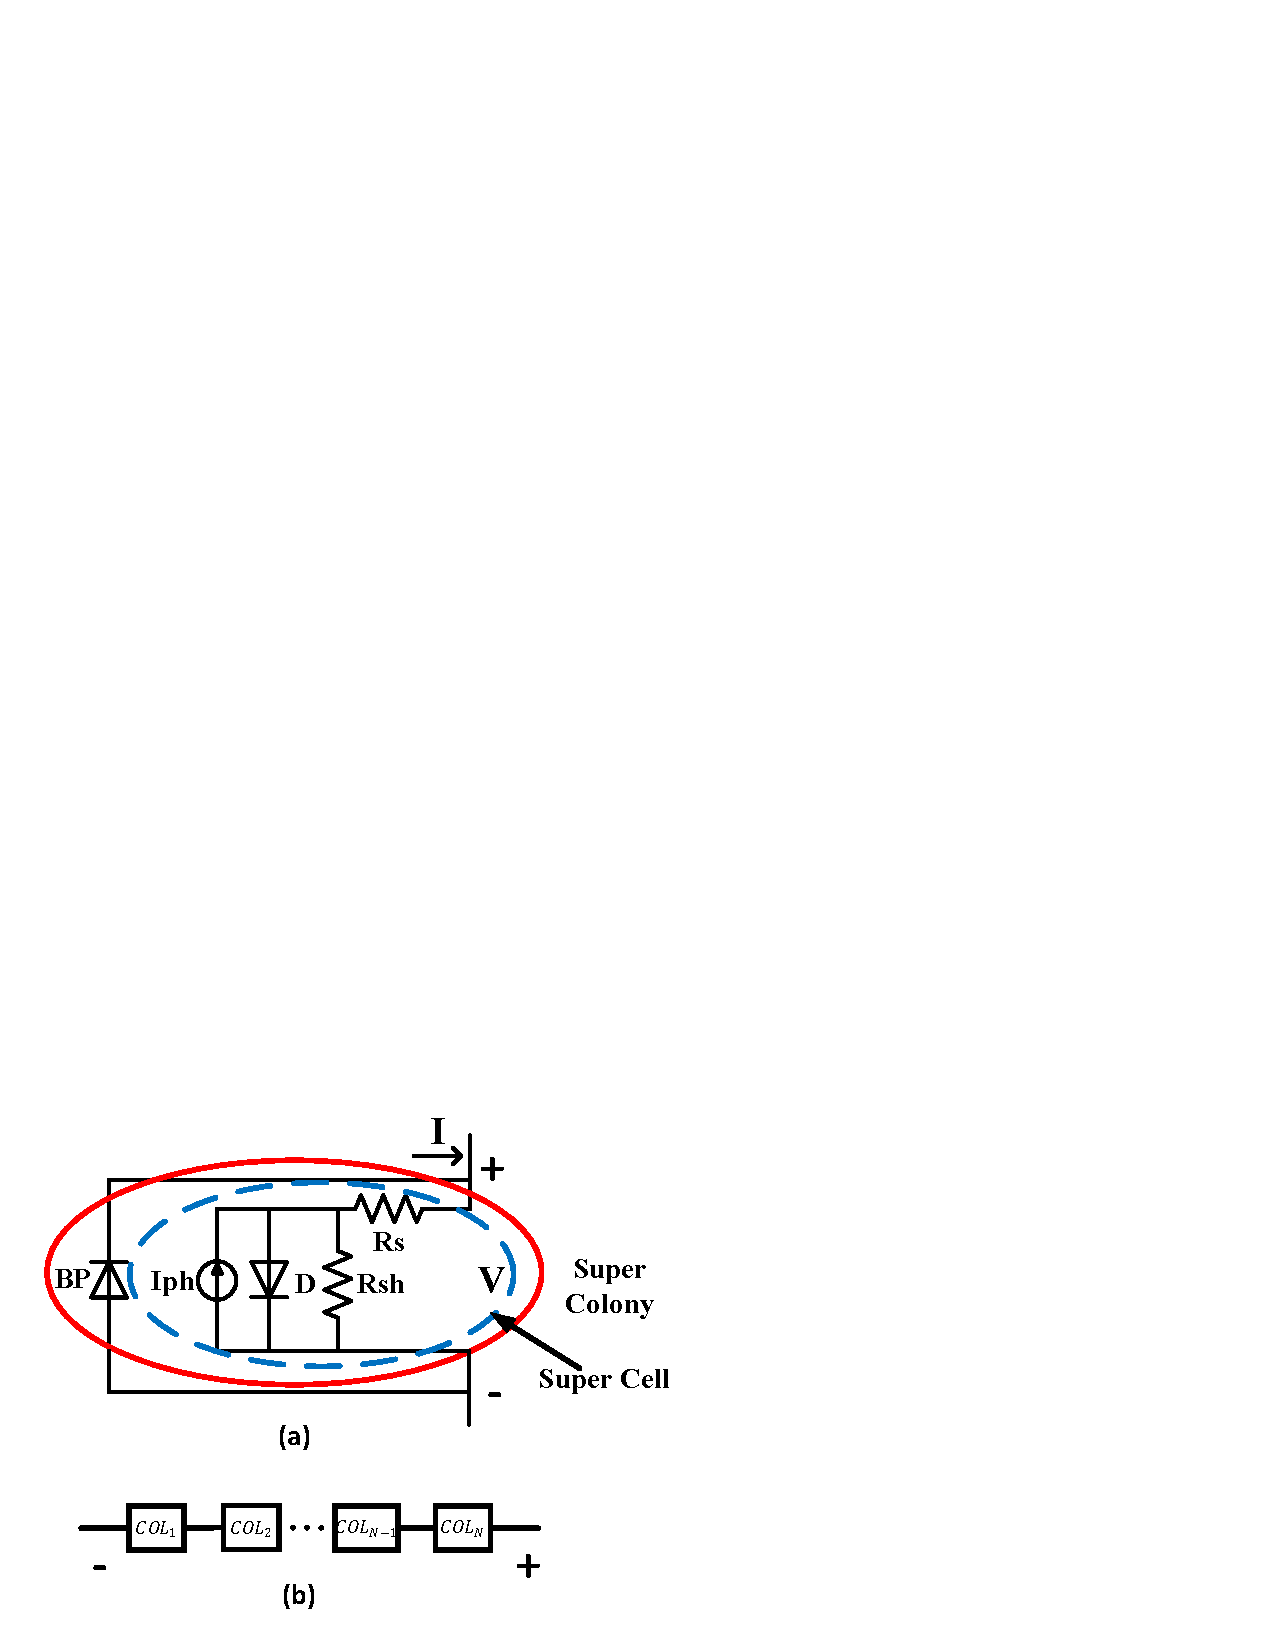
\includegraphics[width=1\columnwidth]{figs/nc_model_diagram.pdf}
    \caption{(a) Equivalent circuit of one super colony in the N-Colony model (b) Diagram of the N-Colony model of a PV module}
    \label{fig:ncDiagram}
\end{figure}

The N-Colony Model consists of $N$  \textit{super colonies}. Each super colony consists of one bypass diode and one \textit{super cell}. The super sell is as circled in Figure \ref{fig:ncDiagram}, and is again modeled by the One-Diode Model. The equivalent circuit diagram for one such colony is shown in Figure \ref{fig:ncDiagram} (a). The N-Colony model of a $mSnP$ PV module is as shown in Figure \ref{fig:ncDiagram} (b).

The N-Colony model is an heuristic model based on experiments. The parameters of the modeled need to be curve fitted from the Ground Truth model. The details of parameter generation is shown in the next sub-section.
\subsection{Parameter Generation of the N-Colony Model}
\subsubsection{Super Colony's Shading Level Generation}
First, we determine the shading level of each super colony. It is also the $I_{ph}$ of the One-Diode model in the super cell.

According to Equation \ref{equ:slMax} and\ref{equ:slMin}, we can calculate the $SL_{max}^{(i,j)}$ and $SL_{min}^{(i,j)}$ of each colony. Note that when the cells are identical within a colony, $SL_{max}^{(i,j)} = SL_{min}^{(i,j)}$ . The notation $(i,j)$ represents the $i^{th}$ colony in the $j^{th}$ column in a PV module.

We define a matrix namely the All Min Matrix ($M_(am)$) to record all $SL_{max}^{(i,j)}$s and $SL_{min}^{(i,j)}$s. $M_(am)$ is an ordered matrix, and is formed as the following. For the $j^{th}$ chain of a PV module, we have the a SL sequence for all the colonies within this chain: $SL_{min}^{(1,j)},SL_{min}^{(2,j)}m \dots,SL_{min}^{(n_{bp},j)}$. We then reorder this sequence into: $SL^{(1,j)},SL^{(2,j)}, \dots,SL^{(n_{bp},j)}$, such that:
\begin{equation}\label{equ:slChain}
  SL^{(1,j)} \le SL^{(2,j)} \le \dots \le SL^{(n_{bp},j)}
\end{equation}
The All Min Matrix then is defined accordingly:
\begin{equation}\label{equ:Mam}
M_{am} =
\begin{bmatrix}
 SL^{(1,1)} & \dots & SL^{(1,n)} \\
 \dots & \dots & \dots \\
 SL^{(n_{bp},1)} & \dots & SL^{(n_{bp},n)} \\
\end{bmatrix}
\end{equation}
where $n$ is the number of chain in a $mSnP$ PV module.

Finally, for the $i^{th}$ super colony in the N-Colony model, its $I_{ph}^i$ is generate by Equation \ref{equ:scIph}:
\begin{equation}\label{equ:scIph}
  I_{ph}^i = \sum_{j=1}^n{M_{am}(i,j)}
\end{equation}

\subsubsection{Cell Shading Ratio, Colony Shading Ratio and Shading Ratio}
We define three variables: the Cell Shading Ratio ($c_r$), the Colony Shading Ratio ($C_R$) and Shading Ratio ($R$) of a N-Colony model. Parameters in N-Colony are generated from $R$, and $R$ depends on $c_r$ and $C_R$. For a PV module that has $n_{bp}$ bypass diodes in a solar cell chain, we have $c_r^1, c_r^2, \dots, c_r^{n_{bp}}$, $C_R^1,C_R^2,\dots,C_R^{n_{bp}}$ and $R^1,R^2,\dots,R^{n_{bp}}$ for a PV module.

$c_r$ and $C_R$ are defined as in Equation \ref{equ:crCR}:
\begin{equation}\label{equ:crCR}
\begin{aligned}
  c_r^i & = \frac{\#i^{th}\ lv\ cell}{m*n} \\
  C_R^i & = \frac{\#i^{th}\ lv\ colony}{n*n_{bp}}
\end{aligned}
\end{equation}
where $\#i^{th}\ lv\ cell$ is the number of solar cells with shading level $i$. A solar cell has shading level $i$ when its SL satisfies:
\begin{equation}\label{equ:ithSLCell}
M_{am} (i-1, j) \ge SL \ge M_{am} (i, j)
\end{equation}
where $j$ is the column this solar cell belongs to.

Similarly, $\#i^{th}\ lv\ colony$ is the number of colonies with shading level $i$, which is defined as in Equation \ref{equ:ithSLCol} :
\begin{equation}\label{equ:ithSLCol}
M_{am} (i-1, j) \ge SL_{min} \ge M_{am} (i, j)
\end{equation}
where $j$ is the column this colony cell belongs to, and $SL_min$ is defined in Equation \ref{equ:slMin}.

$R$ is defined as:
\begin{equation}\label{equ:rDef}
R^i =
    \begin{cases}
      \alpha_i*c_r^i+ \beta_i*C_R^i+ \gamma_i  & \text{if}\  i \neq n_{bp}\\
      1 - \sum_{j = 1}^{n_{bp}-1}{R^i} & \text{otherwise}
     \end{cases}
\end{equation}
where $\alpha_i$, $\beta_i$ and $\gamma_i$ are the weighing factors that need to be curve fitted. Note that we need to make sure all $R^i$s are greater then zero.

Therefore, for a PV module with $n*n_{bp}$ bypass diodes on each chain, $(n*n_{bp} - 1)*3$ parameters are required to be curve fitted.

\subsubsection{Parameters in the N-Colony Model}
Once we have all $R^i$s and $I_{ph}^i$s, we can generate all N-Colony model parameters based on Table \ref{table:ncRule}.
\begin{table}[tb]
  \caption{Model Reduction Rule for the N-Colony Model }
  \label{table:ncRule}
  \centering
  \normalsize
\begin{tabular}{|l|l|}
  \hline
  Parameter & Super Colony $i$ \\
  \hline
  $I_{ph}^s$ & $I_{ph}^i$ \\
  \hline
  $I_s^s$ & $I_{s_o}*n*R^i $\\
  \hline
  $N^s$ & $N_o*m*R^i $\\
  \hline
  $R_s^s$ & $R_{s_o}*m/n*R^i$ \\
  \hline
  $R_{sh}^s$ & $R_{sh_o}/n*R^i$  \\
  \hline
  $I_{s_{bp}}^s$ & $I_{s_{bp_o}}*n*R^i$  \\
  \hline
  $N_{bp}^s$ & $N_{bp_o}*n*R^i$  \\
  \hline
\end{tabular}
\end{table}
In Table \ref{table:ncRule} $I_{s_{bp}}^s$ and $N_{bp}^s$ are the parameters of the bypass diode in the super colony. The superscript $s$ denotes the corresponding parameters are from the super colony.

\begin{table*}[tb]
  \caption{Curve Fitting Results of the N-Colony Model}
  \label{table:ncCurveFit}
  \centering
  \normalsize
\begin{tabular}{|l|l|l|l|}
  \hline
  Weighting Factors & $60s2p$ & $30s4p$ & $40s2p$\\
  \hline
  $\{\alpha_1, \beta_1, \gamma_1\}$ &$\{0.41, 0.17, 0.04\} $ & $\{0.39, 0.19, 0.09\} $ & $\{0.37, 0.17, 0.06\}$ \\
  \hline
  $\{\alpha_2, \beta_2, \gamma_2\}$ &$\{0.40, 0.20, 0.14\} $ & $\{0.41, 0.20, 0.09\} $ & $\{0.41, 0.20, 0.07\}$ \\
  \hline
\end{tabular}
\end{table*}


\subsubsection{Curve Fitting of the Weighting Factors}
The goal of the N-Colony model is to minimize the error between its Power-Voltage (PV) curve and the curve generated by the Ground Truth model. In addition, we care about the maximum power point (MPP), which is the optimal operation point of a PV module. Therefore, the objective function of the curve fitting is described in Equation \ref{equ:cfObj}.
\begin{equation}\label{equ:cfObj}
Obj = w_1*0.5*(2-CORR)+ w_2*Error_{MPP}
\end{equation}
where $Error_{MPP}$ is the relative error of the maximum power point (MPP) and CORR is the correlation of the two curves. If we have two P-V curves, namely $X$ and $Y$, with each curve consisting of sampled points $x_i$ and $y_i$, $i=1,2,\dots,n$, then the CORR of the two curves is defined in Equation \ref{equ:corrDef}.
\begin{equation}\label{equ:corrDef}
CORR = \frac{\sum_{i=1}^n{(x_i - \bar{x})(y_i - \bar{y}) } } {\sqrt{\sum_{i=1}^n{(x_i - \bar{x})^2}}\sqrt{\sum_{i=1}^n{(y_i - \bar{y})^2}}}
\end{equation}
where $\bar{x}$ and $\bar{y}$ are the average value for all $x_i$ and $y_i$. Note that the closer $CORR$ is to $1$, the more similar the two curves are.

In addition, to quantify the impacts of these two optimization goals, they have to be normalized. MPP has already been normalized because its value is between $0$ and $1$. However, CORR has a range between $-1$ and $1$. Therefore, the $0.5*(2-CORR )$ term is the normalization term used in Equation \ref{equ:cfObj}. Furthermore, $w_1$  and $w_2$ are weights that are used to count for the impacts of CORR and MPP after normalization. In our experiment, they are both set to $0.5$ to make the impacts of CORR and MPP equal.

%\subsection{Table-based N-Colony Model}
%The N-Colony model has high efficiency. Furthermore, if there are only $2$ bypass diodes in a solar cell chain, we can build a Table-based N-Colony model.
%
%Under the above assumption when $n_{bp}=2$, only four key variables: $c_r$, $C_R$, $I_{ph}^1$ and $I_{ph}^2$, are enough to derive all parameters in the N-Colony model. For a $mSnP$ PV module, the combination of $c_r$ equals $m*n$, $C_R$ equals $2^{2m}$ and both $I_{ph}^1$ and $I_{ph}^2$ equal $n_{sl}*m$, where $n_{sl}$ is the number of shading levels a PV model have. Therefore, this model can be pre-calculated and stored into a four-dimensional table. In addition, computing time for each variable-combination is constant, which makes the table build-up time to be scalable. For a given shading pattern, the P-V curve can be estimated by table lookup according to the four variables. Fetching data from table needs only a small and constant complexity, which is very efficient.












